\textbf{Chu trình dưới tới hạn cho máy lạnh}\\

Carbon dioxide (\(\mathrm{CO}_2\)) đã từng được sử dụng phổ biến trong các loại máy lạnh và điều hòa vào cuối thế kỉ XIX và đầu thế kỉ XX, trước khi các loại khí ga làm lạnh tổng hợp được phát minh. Trong những năm trở lại đây, khi người ta quan tâm hơn về ảnh hưởng môi trường của các loại ga làm lạnh đang được sử dụng phổ biến, carbon dioxide đang trở lại như một lựa chọn tiềm năng với tác động môi trường thấp, không độc, rẻ và có sẵn, và với những đặc tính nhiệt động và thủy động học có lợi cho thiết kế các hệ thống điều hòa. \\

Chúng ta sẽ cùng khảo sát hoạt động của một hệ thống điều hòa thông dụng ở chế độ dưới bão hòa: Cho \(n\) mol của một loại khí ga thực hiện chu trình như được miêu tả trên đồ thị 1a và 1b, với \(h\) và \(s\) lần lượt là enthalpy và entropy riêng của 1 mol. Lưu ý: hình vẽ không theo tỉ lệ. \\

\begin{center}
    \begin{tikzpicture}
%Đồ thị p-h
  \draw[->] (0,0) -- (6,0) node[below] {$h$};
  
  \draw[->] (0,0) -- (0,4) node[left] {$p$};
  \draw (3,1.5) -- (4.5,3) -- (1,3) -- (1,1.5) -- (3,1.5);
  \draw [dashed] (1,3) -- (0,3);
  \draw [dashed] (1,1.5) -- (0,1.5);
  \filldraw[black] (4,3) circle (1pt);
  \node at (3,1.2) {1};
  \node at (4.5,3.2) {2};
  \node at (4,3.2) {3};
  \node at (1,3.2) {4};
  \node at (1,1.2) {5};
  \node at (-0.3,-0.3) {O};
  \node at (-0.7,3) {$p_{bh}(T_H)$};
  \node at (-0.7,1.5) {$p_{bh}(T_C)$};
    \node at (3,-1) {\textbf{(a)}};
%Đồ thị T-s 
  \draw[->] (8,0) -- (14,0) node[below] {$s$};
  \draw[->] (8,0) -- (8,4) node[left] {$T$};
  \draw (12.5, 1.5) -- (12.5, 3.5);
  \draw plot [smooth, tension = 2] coordinates{(12.5, 3.5) (12.3, 3.2) (12, 3)};
  \draw (12, 3) -- (9,3);
  \draw [dashed] (9,3) -- (10,1.5);
  \draw (10,1.5) -- (12.5,1.5);
  \draw [dashed] (9,3) -- (8,3);
  \draw [dashed] (10,1.5) -- (8,1.5);
  \node at (7.7,-0.3) {O};
  \node at (12.5, 1.2) {1};
  \node at (12.5, 3.7) {2};
  \node at (12, 3.2) {3};
  \node at (9, 3.2) {4};
  \node at (10, 1.2) {5};
  \node at (7.7, 3) {$T_H$};
  \node at (7.7,1.5) {$T_C$};
  \node at (11,-1) {\textbf{(b)}};
\end{tikzpicture} \\
Hình 1: \textbf{(a)} Giản đồ $p-h$ của khí ga. \textbf{(b)} Giản đồ $T-s$ của khí ga.
\end{center}
Chu trình này được mô tả như sau: \\
1-2: Nén khí đoạn nhiệt \\
2-3: Làm mát đẳng áp \\
3-4: Ngưng tụ đẳng nhiệt \\
4-5: Giãn khí đột ngột (Quá trình Joule - Thompson) \\
5-1: Bay hơi đẳng nhiệt \\

Áp suất hơi bão hòa tại nhiệt độ \(T_H\), \(T_C\), enthalpy riêng của pha lỏng, nhiệt hóa hơi mol của pha lỏng coi như đã biết. Giả sử rằng ở thể hơi, khí ga này là một khí lý tưởng đa nguyên tử.
\begin{enumerate}
    \item Tìm nhiệt độ \(T_2\) theo \(T_C\), \(p_{bh}(T_C)\), \(p_{bh}(T_H)\).
    \item Tìm nhiệt lượng do ga tỏa ra trong quá trình 2-3 và 3-4.
    \item Quá trình giãn khí là một quá trình xảy ra rất nhanh, khi đó ta có thể bỏ qua sự trao đổi nhiệt của ga với môi trường trong quá trình này. Thừa nhận rằng tổng enthalpy của ga không đổi trong quá trình này. Tìm tỉ lệ mol ga bị hóa hơi ở cuối quá trình 4-5.
    \item Tìm nhiệt lượng khí ga thu vào trong quá trình 5-1.
    \item Tìm công cần cung cấp cho ga để thực hiện một chu trình theo \(T_h\), \(T_c\), \(p_{bh}(T_h)\), \(p_{bh}(T_c)\), \(h(T_H)\), \(h(T_C)\).
    \item Tìm hiệu suất của chu trình.
    \item Áp dụng số cho \(\mathrm{CO}_2\) với \(T_H = \SI{20}{^{\circ} C}\) và \(T_C = \SI{0}{^{\circ} C}\), nhiệt hóa hơi \(L = \SI{16.5}{kJ/mol}\). Vì sao chu trình này với ga \(\mathrm{CO}_2\) lại không được dùng cho điều hòa nhiệt độ tại nhà thông thường?.
\end{enumerate}

% \vspace{3mm}
% Bảng 1: Các thông số nhiệt động lực học của pha lỏng của \(\mathrm{CO}_2\) tại áp suất hơi bão hòa theo nhiệt độ
% \begin{figure}[H]
%     \centering
%     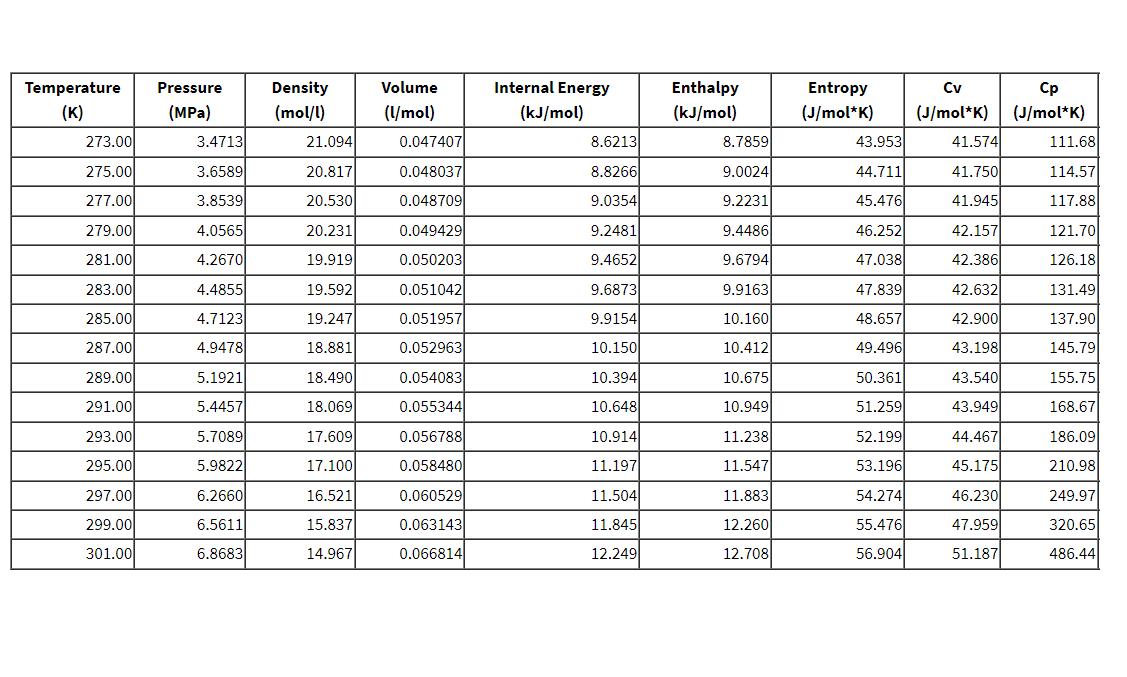
\includegraphics[scale=0.75]{Problem_2/Liquid_phase.png}
    
%     \label{fig:enter-label}
% \end{figure}

\begin{center}
\footnotesize{
\begin{tabular}{|>{\centering\arraybackslash}m{2cm}|>{\centering\arraybackslash}m{2cm}|>{\centering\arraybackslash}m{2cm}|>{\centering\arraybackslash}m{2cm}|>{\centering\arraybackslash}m{2cm}|>{\centering\arraybackslash}m{2cm}|}
    \hline
    Nhiệt độ & Áp suất & Mật độ mol & Nội năng & Enthalpy & Entropy \\
    $(\si{K})$ & $(\si{MPa})$ & $(\si{mol/l})$ & $(\si{kJ/mol})$ & $(\si{J/mol \cdot K})$ & $(\si{J/mol \cdot K})$ \\
    \hline
    273.00 & 3.4713 & 21.094 & 8.6213 & 8.7859 & 43.953 \\
    \hline
    275.00 & 3.6589 & 20.817 & 8.8266 & 9.0024 & 44.711 \\
    \hline
    277.00 & 3.8539 & 20.530 & 9.0354 & 9.2231 & 45.476 \\
    \hline
    279.00 & 4.0565 & 20.231 & 9.2481 & 9.4486 & 46.252 \\
    \hline
    281.00 & 4.2670 & 19.919 & 9.4652 & 9.6794 & 47.038 \\
    \hline
    283.00 & 4.4855 & 19.592 & 9.6873 & 9.9163 & 47.839 \\
    \hline
    285.00 & 4.7123 & 19.247 & 9.9154 & 10.160 & 48.657 \\
    \hline
    287.00 & 4.9478 & 18.881 & 10.150 & 10.412 & 49.496 \\
    \hline
    289.00 & 5.2921 & 18.490 & 10.394 & 10.675 & 50.361 \\
    \hline
    291.00 & 5.4457 & 18.069 & 10.648 & 10.949 & 51.259 \\
    \hline
    293.00 & 5.7089 & 17.609 & 10.914 & 11.238 & 52.199 \\
    \hline
    295.00 & 5.9822 & 17.100 & 11.197 & 11.547 & 53.196 \\
    \hline
    297.00 & 6.2660 & 16.521 & 11.504 & 11.883 & 54.274 \\
    \hline
    299.00 & 6.5611 & 15.837 & 11.845 & 12.260 & 55.476 \\
    \hline
    301.00 & 6.8683 & 14.967 & 12.249 & 12.708 & 56.904 \\
    \hline
\end{tabular}
}
\end{center}

\begin{flushright}
    (Biên soạn bởi Yuki)
\end{flushright}